\section{Method}
\label{sec:method}

\begin{figure*}[t]
\centering
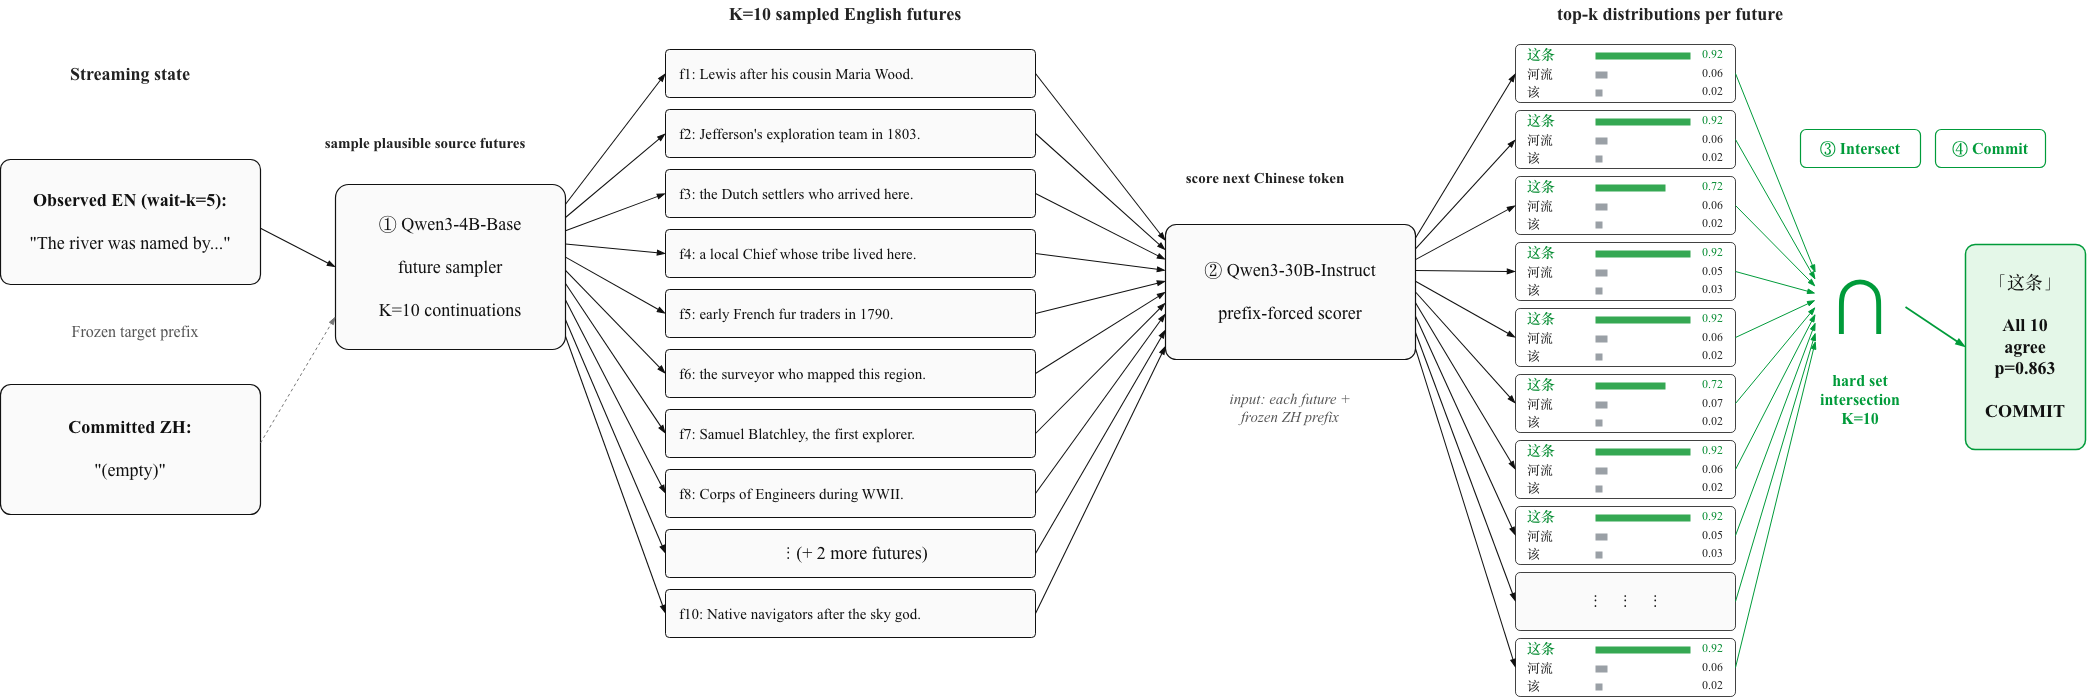
\includegraphics[width=\textwidth]{figures/consensus_decoding.drawio.png}
\caption{Overview of future-conditioned consensus decoding. Given an observed source prefix, multiple base language models sample plausible source continuations. An instruction-tuned translation model is queried in parallel for next-token distributions conditioned on each hypothesised full source and the committed target prefix. The intersection of per-future candidate sets (top-$k$ / min-$p$ / top-$p$) yields a consensus token, which is appended to a pending buffer; the loop repeats until the intersection becomes empty. The committed token-ids are kept exactly as produced by the model, with a final byte-boundary trim before they are written out as supervision.}
\label{fig:pipeline}
\end{figure*}

\subsection{Problem Formulation}

Define $\mathbf{x}_{1:j} = (x_1, \dots, x_j)$ as the partial source text observed
so far and $\mathbf{y}_{1:i} = (y_1, \dots, y_i)$ as the target hypothesis already
committed. Let $g_i$ denote the number of source tokens read before
generating target token $y_i$. A simultaneous translation policy
$\pi(\mathbf{x}_{1:j}, \mathbf{y}_{1:i}) \in [0, 1]$ determines the probability
of emitting a target token (WRITE) versus consuming the next source token
(READ). The complete simultaneous translation process can be formulated as:
\begin{equation}
\small
\begin{aligned}
P(\mathbf{y}, \mathbf{g} \mid \mathbf{x})
&= \prod_{i=1}^{|\mathbf{y}|} \Bigg[
   P_{MT}\!\left(y_i \mid \mathbf{x}_{1:g_i}, \mathbf{y}_{1:i-1}\right)
   \,\pi\!\left(\mathbf{x}_{1:g_i}, \mathbf{y}_{1:i-1}\right) \\
&\qquad\qquad\qquad\;\times
   \prod_{j=g_{i-1}}^{g_i - 1}
   \left(1 - \pi\!\left(\mathbf{x}_{1:j}, \mathbf{y}_{1:i-1}\right)\right)
   \Bigg].
\end{aligned}
\normalsize
\end{equation}

Translation quality is assessed by comparing $\mathbf{y}$ to a reference
$\mathbf{y}^*$ using a metric $Q(\mathbf{y}, \mathbf{y}^*)$, and latency is
measured by a function $L(\mathbf{x}, \mathbf{y}, \mathbf{y}^*, \mathbf{g})$
such as Average Lagging or its length-adaptive
variant.

\subsection{Oracle Future-Conditioned Translation}

In offline translation the full source $\mathbf{x}_{1:J}$ is available and the
translation model can condition on it entirely. In simultaneous translation,
however, only $\mathbf{x}_{1:j}$ has been observed at decision time. An oracle
simultaneous translation model would marginalize over all possible future
source continuations:
\begin{equation}
\begin{aligned}
P^*_{MT}\!\left(y_{i+1} \mid \mathbf{x}_{1:j}, \mathbf{y}_{1:i}\right)
&= \\
\mathbb{E}_{\substack{\mathbf{x}_{j+1:}\,\sim\\[-0.2ex] P^*_{LM}(\cdot \mid \mathbf{x}_{1:j})}}
\Bigl[
&\quad P^*_{MT}\!\left(y_{i+1} \mid \mathbf{x}_{1:j}, \mathbf{x}_{j+1:}, \mathbf{y}_{1:i}\right)
\Bigr].
\end{aligned}
\label{eq:oracle}
\end{equation}
where $P^*_{LM}(\cdot \mid \mathbf{x}_{1:j})$ is the true distribution over
future source tokens. Direct computation of Eq.~\ref{eq:oracle} is intractable
since it requires marginalizing over all possible future source sequences. We
approximate it in two ways: (1)~replacing $P^*_{LM}$ with Monte Carlo samples
from a base language model, and (2)~replacing the soft expectation with a
conservative \emph{consensus} operation that commits only to tokens on which
all sampled futures agree.

\subsection{Future-Conditioned Consensus Decoding}

At each streaming step the system observes a partial source prefix
$\mathbf{x}_{1:t}$ and has already committed a target token-id sequence
$\mathbf{y}_{<i}$.

\paragraph{Step 1: Future Sampling.}
We sample $M$ plausible source continuations
$\{\hat{\mathbf{x}}^{(m)}\}_{m=1}^{M}$ from \emph{two heterogeneous} base
language models---a smaller and a larger pretrained base LM---by prompting
each with $\mathbf{x}_{1:t}$ and drawing continuations of up to $T$ tokens
with temperature $\tau$. Using two architecturally different bases is
deliberate: drawing all futures from a single LM tends to produce
self-agreement (the consensus collapses to the model's own bias), whereas
heterogeneous bases force the consensus to rely on signal that is robust
across model families. Each continuation is concatenated with the observed
prefix to form a hypothetical full source context
$\tilde{\mathbf{x}}^{(m)} = \mathbf{x}_{1:t} \oplus \hat{\mathbf{x}}^{(m)}$.

\paragraph{Step 2: Next-Token Distribution Probing.}
For each hypothetical source $\tilde{\mathbf{x}}^{(m)}$, we query an
instruction-tuned translation model with a prompt containing
$\tilde{\mathbf{x}}^{(m)}$ and the committed target prefix
$\mathbf{y}_{<i}$, requesting only a single token with its top-$K$
log-probabilities. This yields a distribution
$D_m = \{(t_k, p_k)\}_{k=1}^{K}$ over next target tokens. Distributions
from all futures are queried in a single batched API call for efficiency.

\paragraph{Step 3: Consensus Token Selection.}
From each distribution $D_m$ we extract a candidate set $C_m$. Three
strategies are supported:
\begin{itemize}
\item \textbf{Top-$k$}: $C_m$ contains the $k$ highest-probability tokens.
\item \textbf{Min-$p$}: $C_m$ contains all tokens whose probability exceeds
      an absolute threshold $p_{\min}$, i.e.\
      $C_m = \{t : D_m(t) \ge p_{\min}\}$.
\item \textbf{Top-$p$} (nucleus): $C_m$ is the smallest set of
      highest-probability tokens whose cumulative probability mass is at
      least $p$, i.e.\ $C_m$ is the minimal prefix of the probability-sorted
      vocabulary such that $\sum_{t \in C_m} D_m(t) \ge p$.
\end{itemize}
We compute the consensus set
\begin{equation}
C = \bigcap_{m=1}^{M} C_m.
\end{equation}
If $C \neq \emptyset$, we select the token with the highest average
probability across futures:
\begin{equation}
y^* = \arg\max_{t \,\in\, C} \; \frac{1}{M} \sum_{m=1}^{M} D_m(t),
\end{equation}
and append its token id to a pending buffer. Steps~2--3 repeat with the
extended prefix until $C = \emptyset$ or a maximum number of consensus steps
is reached.

\paragraph{Step 4: Minimum-Horizon Filter.}
A short-lived consensus is fragile evidence: if the loop breaks after only
one or two confirmed tokens, the path is likely to lock the system into a
translation that the next source chunk would have invalidated. We therefore
apply a minimum-horizon filter: if $|\text{pending}| < h_{\min}$, the entire
pending buffer is discarded and the system falls through to a READ. This
trades a small amount of incremental progress for a large reduction in
catastrophic early-commit errors.

\paragraph{Step 5: Commitment.}
After the consensus loop terminates, if the pending buffer survives the
horizon filter, its contents are committed as a WRITE action; otherwise the
decoder performs a READ, reads one additional source chunk, and re-enters
Step 1. When the final source chunk arrives, the consensus loop is bypassed
and the instruction-tuned model generates the remaining translation in a
single completion call, ensuring every utterance receives a complete
translation.

\subsection{Decoding in Token-ID Space}

A naive implementation of the loop would, at every step, decode the pending
buffer to text and re-encode it as part of the next prompt. For byte-level
BPE tokenizers this round-trip is unsafe: CJK characters are typically
emitted as multi-byte token sequences, and adjacent tokens such as
\texttt{["而", "且"]} can be re-merged on re-encoding into a single token
\texttt{["而且"]}, silently shifting the model state away from the
trajectory that produced the consensus.

We therefore maintain the entire committed and pending continuation as a
sequence of token ids and feed it directly to the instruction-tuned model
as a token-id prefix, never round-tripping through text. Two safeguards
are applied at the boundary between the pending buffer and a WRITE action:
(i)~tokens that the tokenizer marks as disallowed for generation (special
tokens, prompt-template fragments) are filtered out and logged; and
(ii)~the longest prefix of the pending buffer whose decoded text contains
no Unicode replacement characters (\texttt{U+FFFD}) or dangling combining
marks is identified, and only that prefix is committed---trailing byte-token
fragments that do not yet form complete characters are kept as state for
the next chunk rather than written out as supervision.

\subsection{Training Data Synthesis Pipeline}

Given an offline parallel corpus with source transcripts and reference
translations, we apply the consensus decoding procedure above to each
utterance. The source transcript is pre-segmented into chunks
$\{c_1, \dots, c_N\}$ simulating incremental speech recognition output.
For each chunk $c_t$ (except the last), the consensus decoder produces a
target delta $\delta_t$ and an action $a_t \in \{\text{READ}, \text{WRITE}\}$.
The resulting trajectory
$\{(c_t, \delta_t, a_t)\}_{t=1}^{N}$ serves as a training example for the
SimulST model.

To ensure translation quality, we score each synthesized example using
MetricX-24 in quality-estimation mode, which evaluates translation
adequacy from source and hypothesis alone without requiring a reference.
Examples whose QE score exceeds a threshold $\theta$ are discarded. The
filtered dataset is then used to train the SimulST model via standard
sequence-to-sequence fine-tuning, producing a model that has internalized
future-aware commitment decisions without requiring LLM calls at inference
time.
